%\documentclass[conference]{IEEEtran}
\documentclass[12pt, onecolumn]{IEEEtran}
\usepackage{graphics,  color,  amsmath, amsfonts, amssymb, balance,algorithm,algorithmic,array ,comment}
\usepackage{graphicx}
%\usepackage{bbding}
%\usepackage{multirow}
\usepackage{caption}
\usepackage{algorithm}
\usepackage{algorithmic}
\usepackage{amsmath, amssymb}
\usepackage{mathrsfs}
\usepackage{bm}%Greek letters in boldface
\vfuzz2pt % Don't report over-full v-boxes if over-edge is small draftcls
\hfuzz2pt % Don't report over-full h-boxes if over-edge is small
% THEOREMS -------------------------------------------------------
\newtheorem{thm}{Theorem}%[section] ,draftcls
\newtheorem{cor}{Corollary}
\usepackage{amsthm}
\newtheorem{lem}{Lemma}
\newtheorem{prop}{Proposition}
\newtheorem{defn}{Definition}
\newtheorem{rem}{Remark}
\newtheorem{example}{Example}
\newtheorem{theorem}{Theorem}
\renewcommand{\algorithmicrequire}{ \textbf{Initialization:}}
\renewcommand{\algorithmicensure}{ \textbf{Return:}}

\author{Jianxin Dai\\
}
\title{Weekly Report of Interference Alignment }
\begin{document}
\maketitle

\section{Introduction}
Interference Alignment (IA) is a revolutionary wireless transmission strategy that reduces the impact of interference.

\section{Priori Knowledge}
\subsection{Paper}
In the paper \cite{cadambe2008interference}, a centralized scheme is present in the form of closed form expressions for the transmit precoding matrices. However, these solutions suffer from expressions require global channel knowledge which can be an  overwhelming overhead in practice. Secondly, closed form solutions have only been found in certain cases. In general, analytical solutions to interference alignment problem are difficult to obtain and even the feasibility of interference alignment over  a limited number of signalling dimension is an open problem. Thirdly, the result of \cite{cadambe2008interference} are meaningful only at high SNR, and to the best of  our knowledge, their performance  at low/moderate SNR is unknown.


In the paper \cite{gomadam2011distributed}, two  distributed strategies are present. The idea for strategies are  that each iteration, users try to minimize the extent to which their signal leaks into the other users' desired signal subspaces. After the algorithm converges, the IA condition should ideally be satisfied and the desired signal spaces be free of interference.   Relying on reciprocity for precoding over the interference channel, however, has a number of potential drawbacks. Iterating over the air may incur a non-negligible overhead due to the recurring pilot transmissions.

In the paper \cite{maddah2012completely}, authors show that in an MIMO broadcast channel with $K$ transmit antennas and K receivers equipped  with one antenna, $\frac{K}{1+ \frac{1}{2}+...+\frac{1}{K}}$ degrees of freedom is achieve even when the fed back channel state is completely independent of the current state. In this scheme, the transmitters uses the fed back CSI to learn the side information that the receivers receive from previous transmissions rather than to predict the current channel state


In the paper \cite{geraci2017operating}, authors proposed to operate massive Multiple Input Multiple Output (MIMO) cellular Base Stations (BSs) in unlicensed bands (mMIMO-U). they design a procedures required at a cellular BS to guarantee coexistence with nearby WiFi stations in the same piece of unlicensed band via interference alignment technology.  Fig.~\ref{FIG:mMIMO} show the flow of mMIMO-U  proposed.
\begin{figure}[H]
    \centering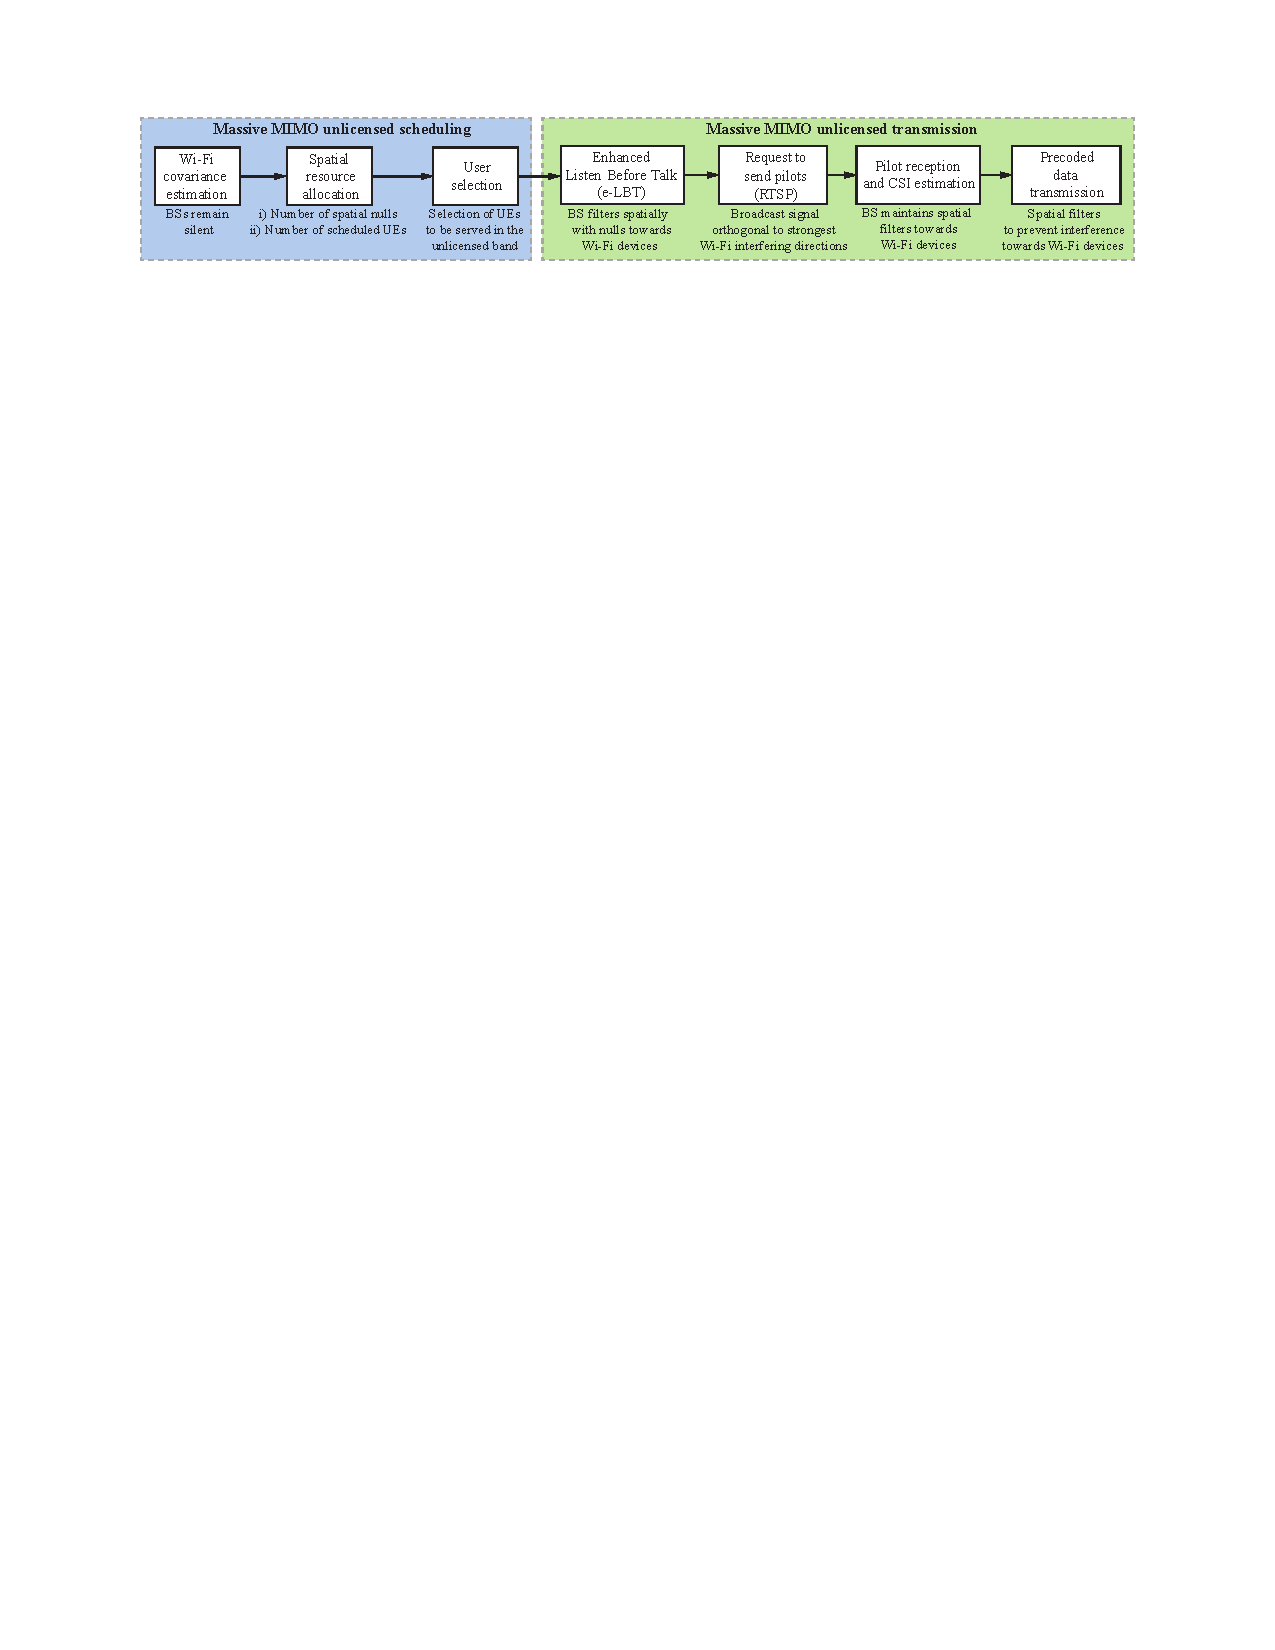
\includegraphics[width=1\columnwidth]{mMIMO.pdf}
    \caption{ Flow chart of the proposed mMIMO-U}\label{FIG:mMIMO}
\end{figure}
\begin{description}
  \item[Step1:] %authors discuss the operations requires for a massive MIMO celluar BS to:
                    \begin{enumerate}
                      \item acquire channel state information from the neighboring WiFi devices.
                      \item allocate spatial resources for WiFi interference suppression and user equipment (UE) multiplexing.
                      \item select a suitable set of UEs to be served in the unlicensed band.
                    \end{enumerate}
  \item[Step2:] %authors devise a transmission operations of a massive MIMO-U system, including:
                    \begin{enumerate}
                        \item an enhanced LBT phase.
                        \item procedures for UE pilot request and channel estimation.
                        \item precoder calculation.
                    \end{enumerate}
\end{description} 
\subsection{Based System Model}
\subsubsection{Channel Transmission}
Consider the $K$-user MIMO interference where the $k^{th}$ transmitter and receiver are equipped with $M$ and $N$ antennas respectively. Note that the channel matrices will have  a diagonal structure. The channel is defined as:
\begin{equation}\label{Channel}
    Y_{[k]} = \sum_{l=1}^{K}H_{[k,l]}X_{[l]} +Z_{[k]}, \qquad  \forall{}k \in \mathcal{K}
\end{equation}
where  $Y_{[k]}$,$Z_{[k]}$ are the $N\times{}1$ received signal vector and the zero mean unit variance circularly symmetric Additive White Gaussian Noise vector(AWGN) at receiver $k$, $X_{[l]}$ is the $M\times{}1$ signal vector transmitted by transmitter $l$, and $H_{[k,l]}$ is the $N\times{}M$ matrix of channel coefficients between transmitter $l$ and receiver $k$. The transmit power at transmitter $l$ is $E[||X_{[l]}||^{2}] = P_{[l]}$. $\mathcal{K} \triangleq \{1,2,...,K\}$ is the index set of K users.


\subsubsection{Precoding at Transmitter}
Let $V_{[k]}$ be an $M\times{}d$ matrix whose columns are the orthonormal basis of of the transmitterd signal space of user k. The degree of freedom can be obtain by $d \leq{} min(M,N)$. Mathematically, the transmitted signal vector of user $k$ is given by:
\begin{equation}\label{Precoding}
    X_{[k]} = V_{[k]}\overline{X}_{[k]}, \qquad \overline{X}_{[k]} \backsim \mathcal{N}(0,\frac{P_{[k]}}{d}\mathbf{I}).
\end{equation}
Each element of the $d\times{}1$ vector $\overline{X}_{[k]}$  represents an independently encode Gaussian codebook symbol with power $\frac{P_{[k]}}{d}$ that is beamformed with the corresponding vector of $V_{[k]}$.


\subsubsection{Interference Suppression at Receiver}
Let $U_{[k]}$ be an $N\times{}d$ matrix whose columns are the orthonormal basis of the interference-free desired signal subspace at receiver $k$. The receiver $k$ filters its  received signal to obtain:
\begin{equation}\label{InterferenceSuppression}
\overline{Y}_{[k]} = U_{[k]}^{\dag}Y_{[k]}
\end{equation}
Then we rewrite the Eq.\eqref{InterferenceSuppression} from Eq.\eqref{Channel} and Eq.\eqref{Precoding}:
\begin{equation}
    \overline{Y}_{[k]} = U_{[k]}^{\dag}H_{[k,k]}V_{[k]}\overline{X}_{[k]} + \sum_{l=1,l\neq{}k}^{K}U_{[k]}^{\dag}H_{[k,l]}V_{[l]}\overline{X}_{[l]} + U_{[k]}^{\dag}Z_{[k]}.
\end{equation}
If  interference is aligned into the null space of $U_{[k]}$ then the following condition must be satisfied:
\begin{eqnarray}
    & U_{[k]}^{\dag}H_{[k,l]}V_{[l]} &= \textbf{0}, \qquad{} \forall l\neq{}k \label{constraint 1} \\
    & \text{rank}(U_{[k]}^{\dag}H_{[k,k]}V_{[k]}) &= d. \label{constraint 2}
\end{eqnarray}
In other words the desired signals are received through a $d\times{}d$ full rank channel matrix:
\begin{equation}
\overline{H}_{[k,k]} \triangleq U_{[k]}^{\dag}H_{[k,k]}V_{[k]},
\end{equation}
while the interference is completely eliminated. The effective channel for user $k$ is then expressed as:
\begin{equation}
\overline{Y}_{[k]}=\overline{H}_{[k,k]} \overline{X}_{[k]}+\overline{Z}_{[k]},
\end{equation}
where $\overline{Z}_{[k]}$ is the effective $d\times{}1$ AWGN vector at receiver $k$. The rate $R_{[k]}$ achieve on this channel is:
\begin{equation}
R_{[k]} = \log(\textbf{I}_{d} + \frac{P_{[k]}}{d}\overline{H}_{[k,k]}\overline{H}_{[k,k]}^{\dag}).
\end{equation}


\subsection{Objective of Interference Alignment}
Given the channel matrices $H_{[k,l]}$, the degrees of freedom $d$ is feasible id there exist transmit precoding matrices $V_{[k]}$ and receive interference suppression matrices $U_{[k]}$ which can satisfy constraint  condition Eq.\eqref{constraint 1} and Eq.\eqref{constraint 2}, such that
\begin{equation}
   \left\{
        \begin{aligned}
                 U_{[k]}^{\dag}H_{[k,l]}V_{[l]} &= \textbf{0}, \qquad{} \forall l\neq{}k  \\
                 \text{rank}(U_{[k]}^{\dag}H_{[k,k]}V_{[k]}) &= d.
        \end{aligned}
   \right.
\end{equation}

\subsection{Scheme of Interference Alignment}
\begin{itemize}
  \item Centralized Scheme
  \item Iterative Interference Alignment
  \item Max-SINR Aligorithm
\end{itemize}

\begin{comment}
\subsection{Centralized Scheme( 3 users with M antenna)}
Let Degrees of Freedom $d = M/2$.  Transmitter $k$ transmits message for receiver $k$ using $M/2$ independently encoded streams.
\begin{equation}
    \begin{aligned}
        \text{span}(H_{[1,2]}V_{[2]}) &= \text{span}(H_{[13]}V_{[3]}) \\
        H_{[1,2]}V_{[2]} &= H_{[13]}V_{[3]} \\
        H_{[1,2]}V_{[2]} &= H_{[13]}V_{[3]}
    \end{aligned}
\end{equation}
where span(A) represent the vector space spanned by the column vectors of matrix A. We now wish to choose the $V_{[k]}$, $k=1,2,3$ so that the above equations are satisfied. Then we can obtain the solution.

\subsection{Distributed Scheme}
\subsubsection{Iterative Interference Alignment}
sss
\begin{algorithm}[H]
\caption{ Iterative Interference Alignment}
\label{alg:Iterative}
\begin{algorithmic}[1]
\STATE Start with arbitrary precoding matrices $V_{[k]}: M\times{}d$,$V_{[k]}^{\dag}V_{[k]}=\mathbf{I}$
\STATE Begin iteration
\STATE Compute interference covariance matrix at the receivers:\\
        $Q_{[k]} = \sum_{j=1,i\neq()k}^{K}\frac{P_{j}}{d}H_{[k,j]}V_{[j]}^{\dag}H_{[k,j]}^{\dag}$
\STATE Compute the interference suppression matrix at each receiver:
        $U_{[k]}^{*i} = v_{i}(Q_{[k]})$ , i  = 1,2...$d$
\STATE Reverse the communication direction and set $V_{[k]} = U_{[k]}$.
\STATE Continue till convergence.
\end{algorithmic}
\end{algorithm}


\subsubsection{Max-SINR Algorithm}
ss
\begin{algorithm}[H]
\caption{ Max-SINR Aligorithm}
\label{alg:Iterative}
\begin{algorithmic}[1]
\STATE Start with arbitrary precoding matrices $V_{[k]}: M\times{}d$ which are linearly independent unit vectors.
\STATE Begin iteration
\STATE Compute interference plus noise covariance matrix for $B_{[k,l]}$ for stream $l$ at receiver $k$.\\
        $B_{[k,l]} = $
\STATE Calculate receive combining vectors
        $U_{[k]}^{*i} = v_{i}(Q_{[k]})$ , i  = 1,2...$d$
\STATE Reverse the communication direction and set $V_{[k]} = U_{[k]}$.
\STATE Continue till convergence.
\end{algorithmic}
\end{algorithm}
\end{comment}



\section{Simulation Work}

\begin{figure}[H]
    \centering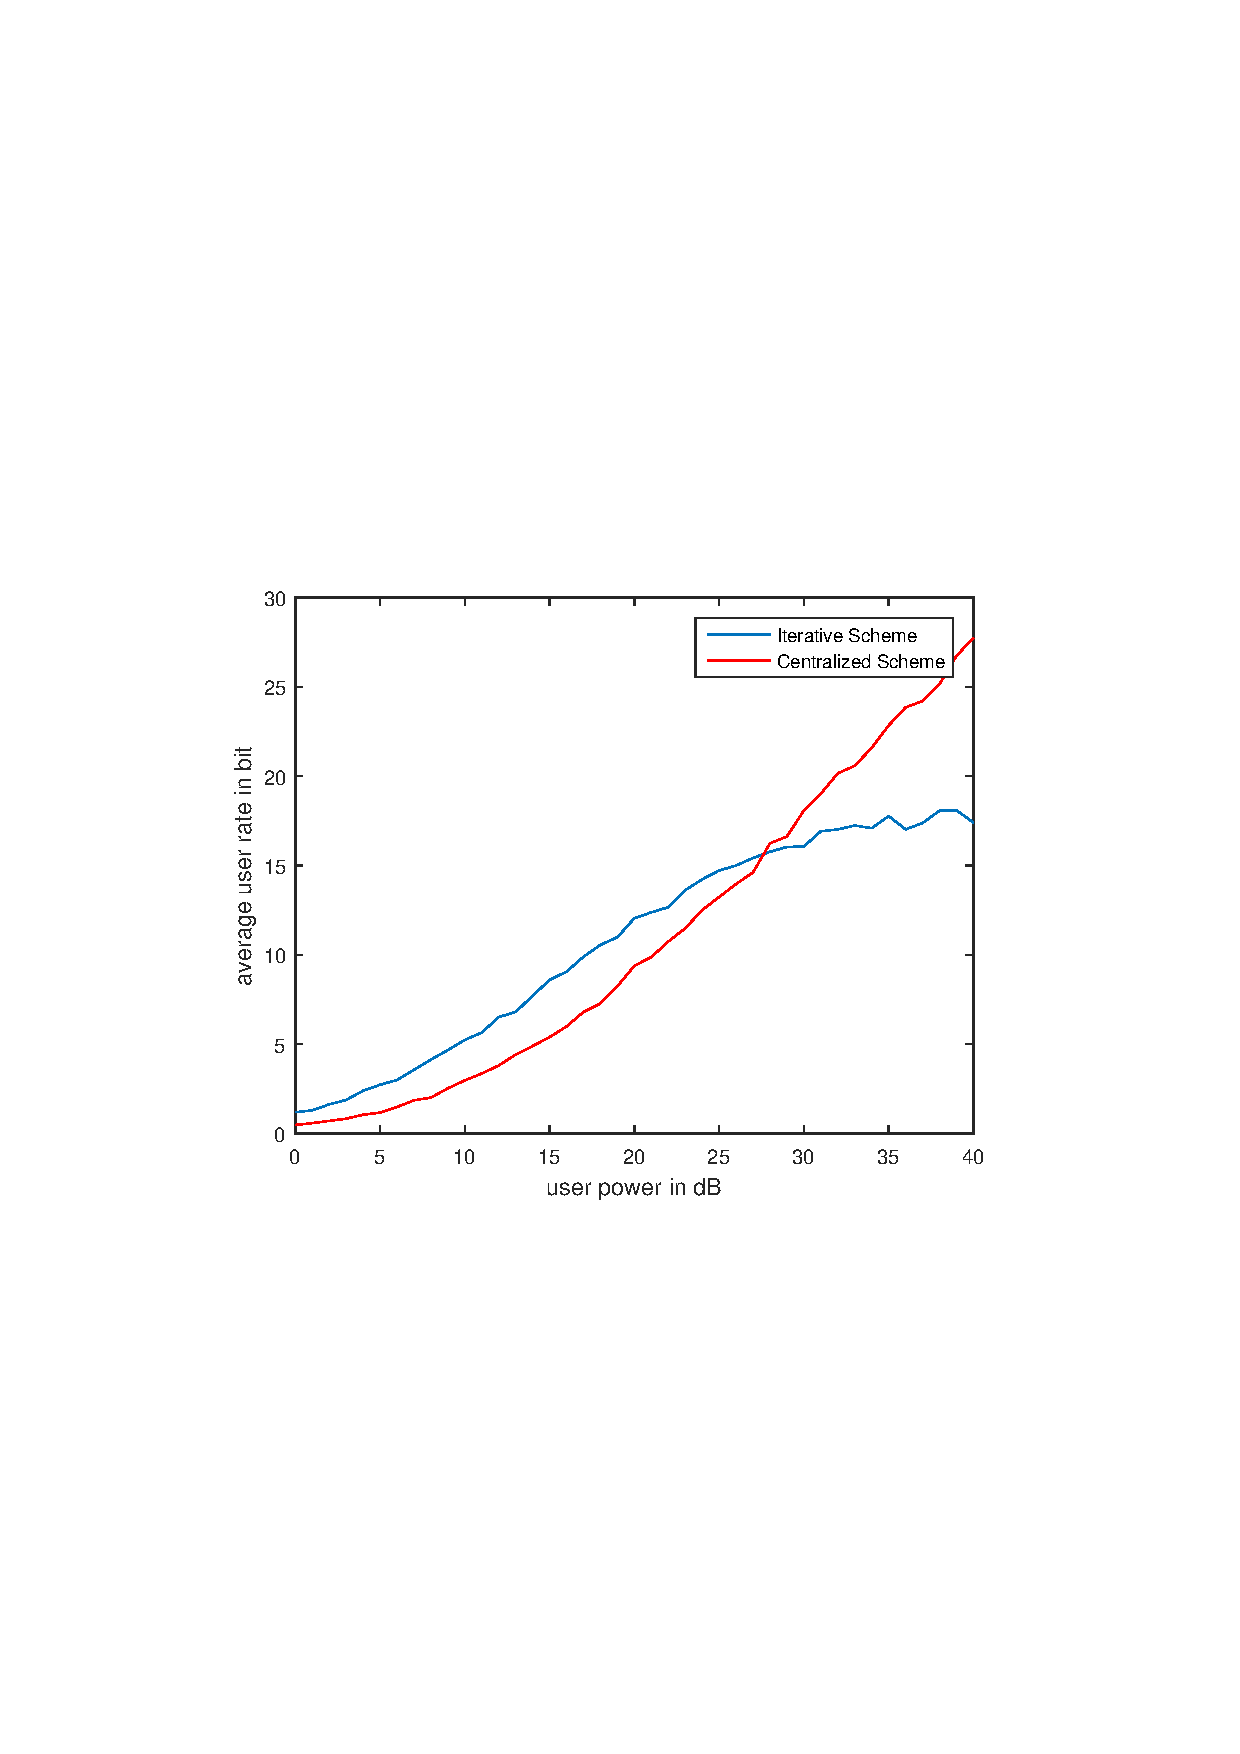
\includegraphics[width=0.6\columnwidth]{result_66.pdf}
    \caption{ Centralized and Distributed Scheme(6,6,3)}\label{FIG:Compare}
\end{figure}

\begin{figure}[H]
    \centering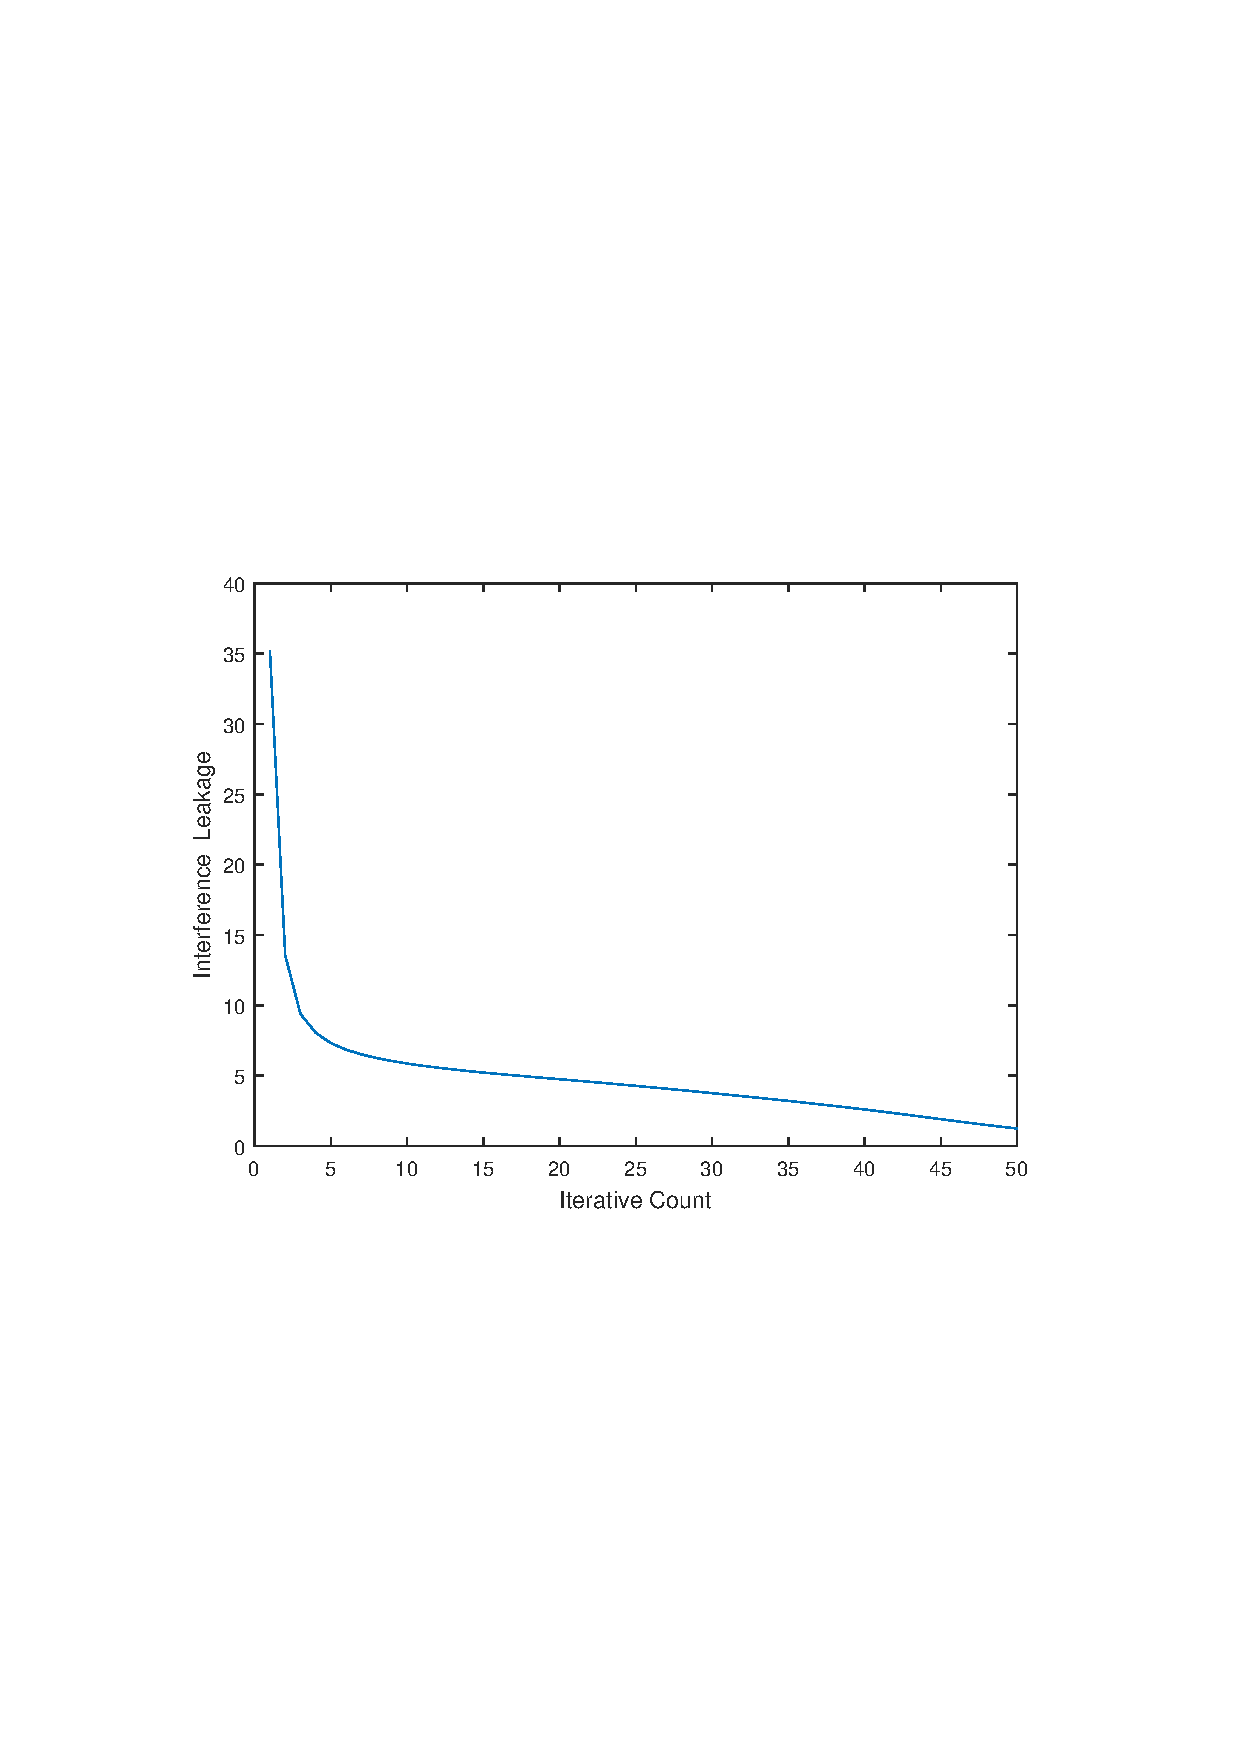
\includegraphics[width=0.65\columnwidth]{IterativeCount.pdf}
    \caption{ Centralized and Distributed Scheme}\label{FIG:IterativeCount}
\end{figure}
For evaluate the performance  of Centralized Scheme \cite{cadambe2008interference} and Distributed Iterative Scheme \cite{gomadam2011distributed}, we do some numerical  simulations with MATLAB. Consider the $3$-user MIMO interference where both of transmitter and receiver are equipped with 6 antennas.  transmission code stream is 3.  The channel matrix $H_{[i,j]}$ is chosen to be independent zero-mean unit-variance i.i.d Gaussian matrix. Meanwhile the noise is  zero mean unit variance  AWGN.   As we can see from Fig.~\ref{FIG:Compare}, the performance of Centralized Scheme will better than  Distributed Iterative Scheme with high user power. It is because that  Iterative Scheme can not eliminate interference from other users completely.   Fig.~\ref{FIG:IterativeCount} shows interference leakage will decrease with a increased iterative count in  Distributed Iterative Scheme .

Similar to \cite{gomadam2011distributed}, we also consider a 3 user interference channel where each node is equipped with 2 antennas and all channel coefficients are i.i.d. zero mean unit variance circularly symmetric complex user achieves 1 degree of freedom. As shown in Fig.~\ref{FIG:result_22},  we compare the performance of the  distributed iterative scheme and centralized scheme.
\begin{figure}[H]
    \centering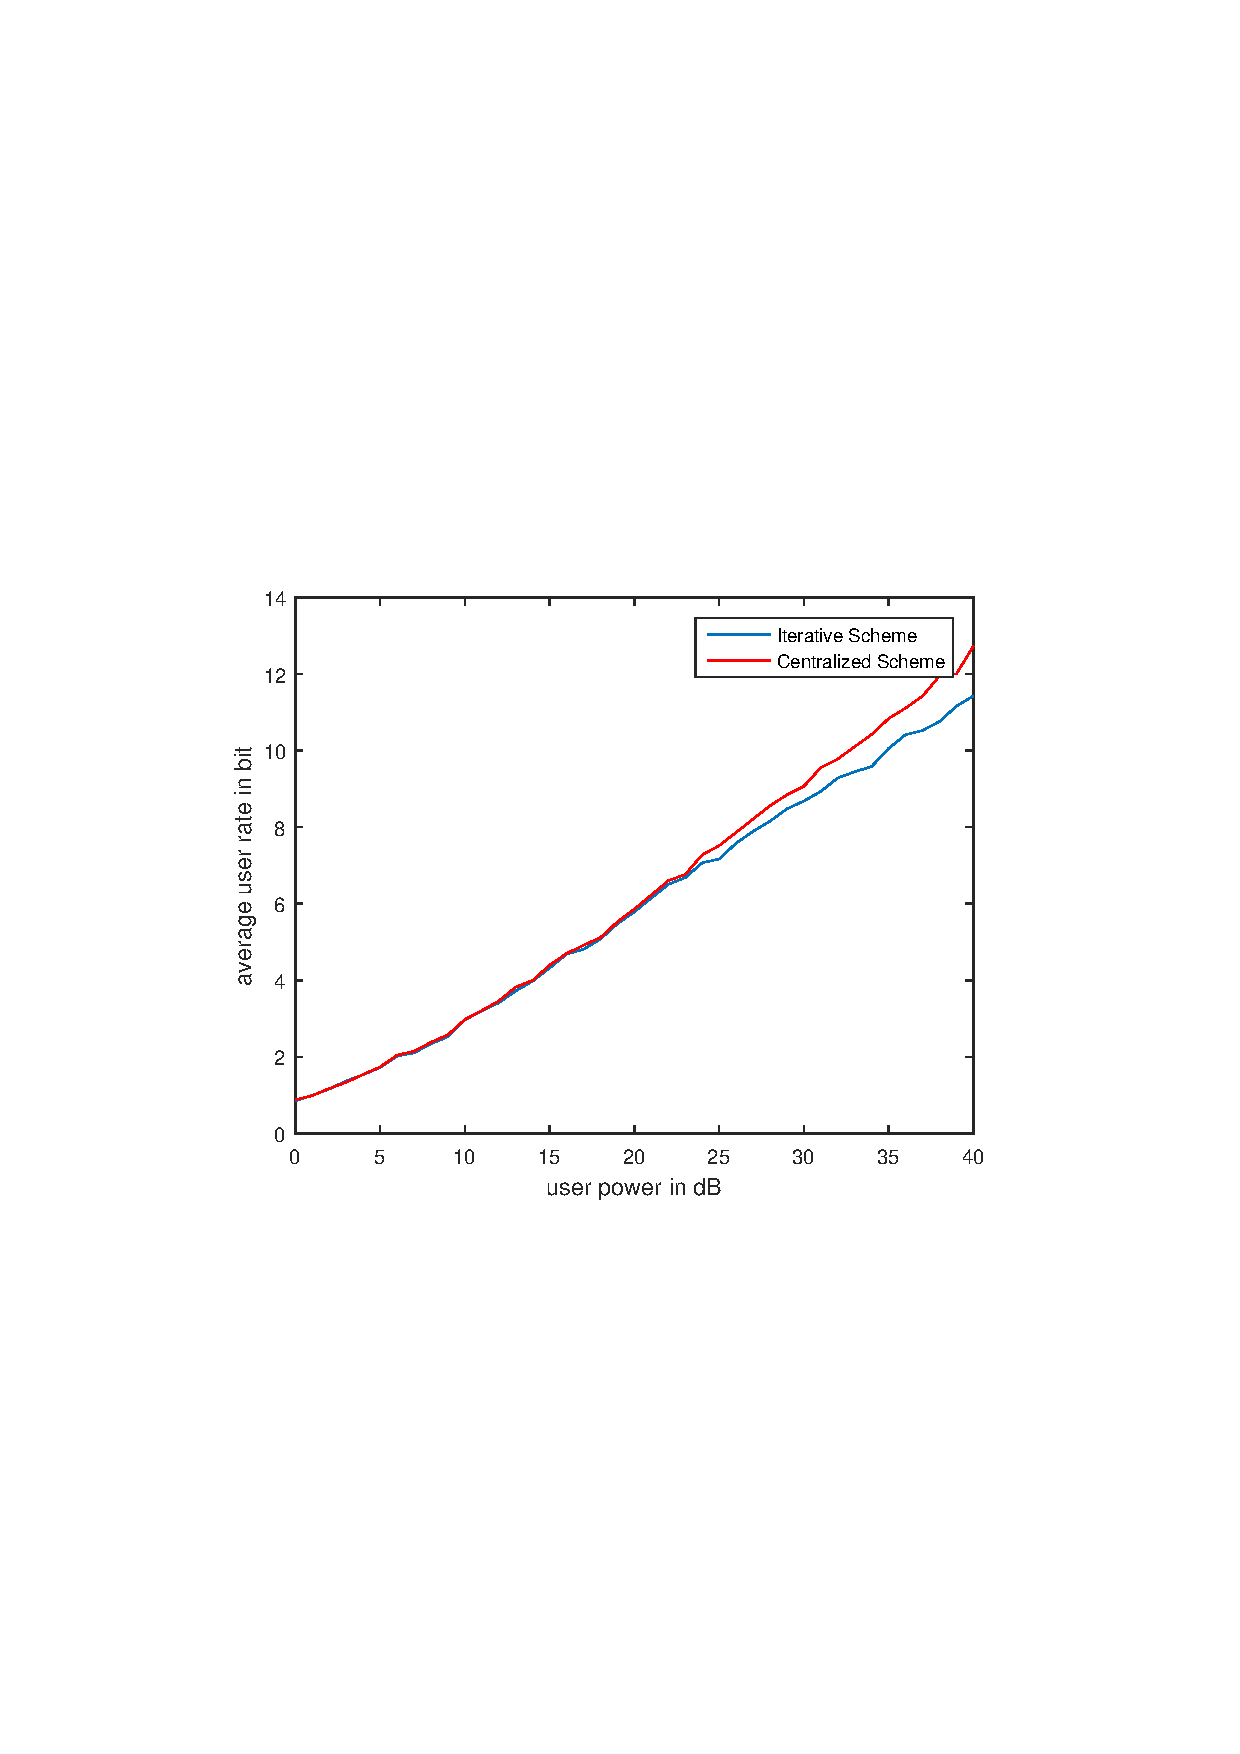
\includegraphics[width=0.65\columnwidth]{result_22.pdf}
    \caption{ Centralized and Distributed Scheme(2,2,1)}\label{FIG:result_22}
\end{figure}
\begin{figure}[H]
    \centering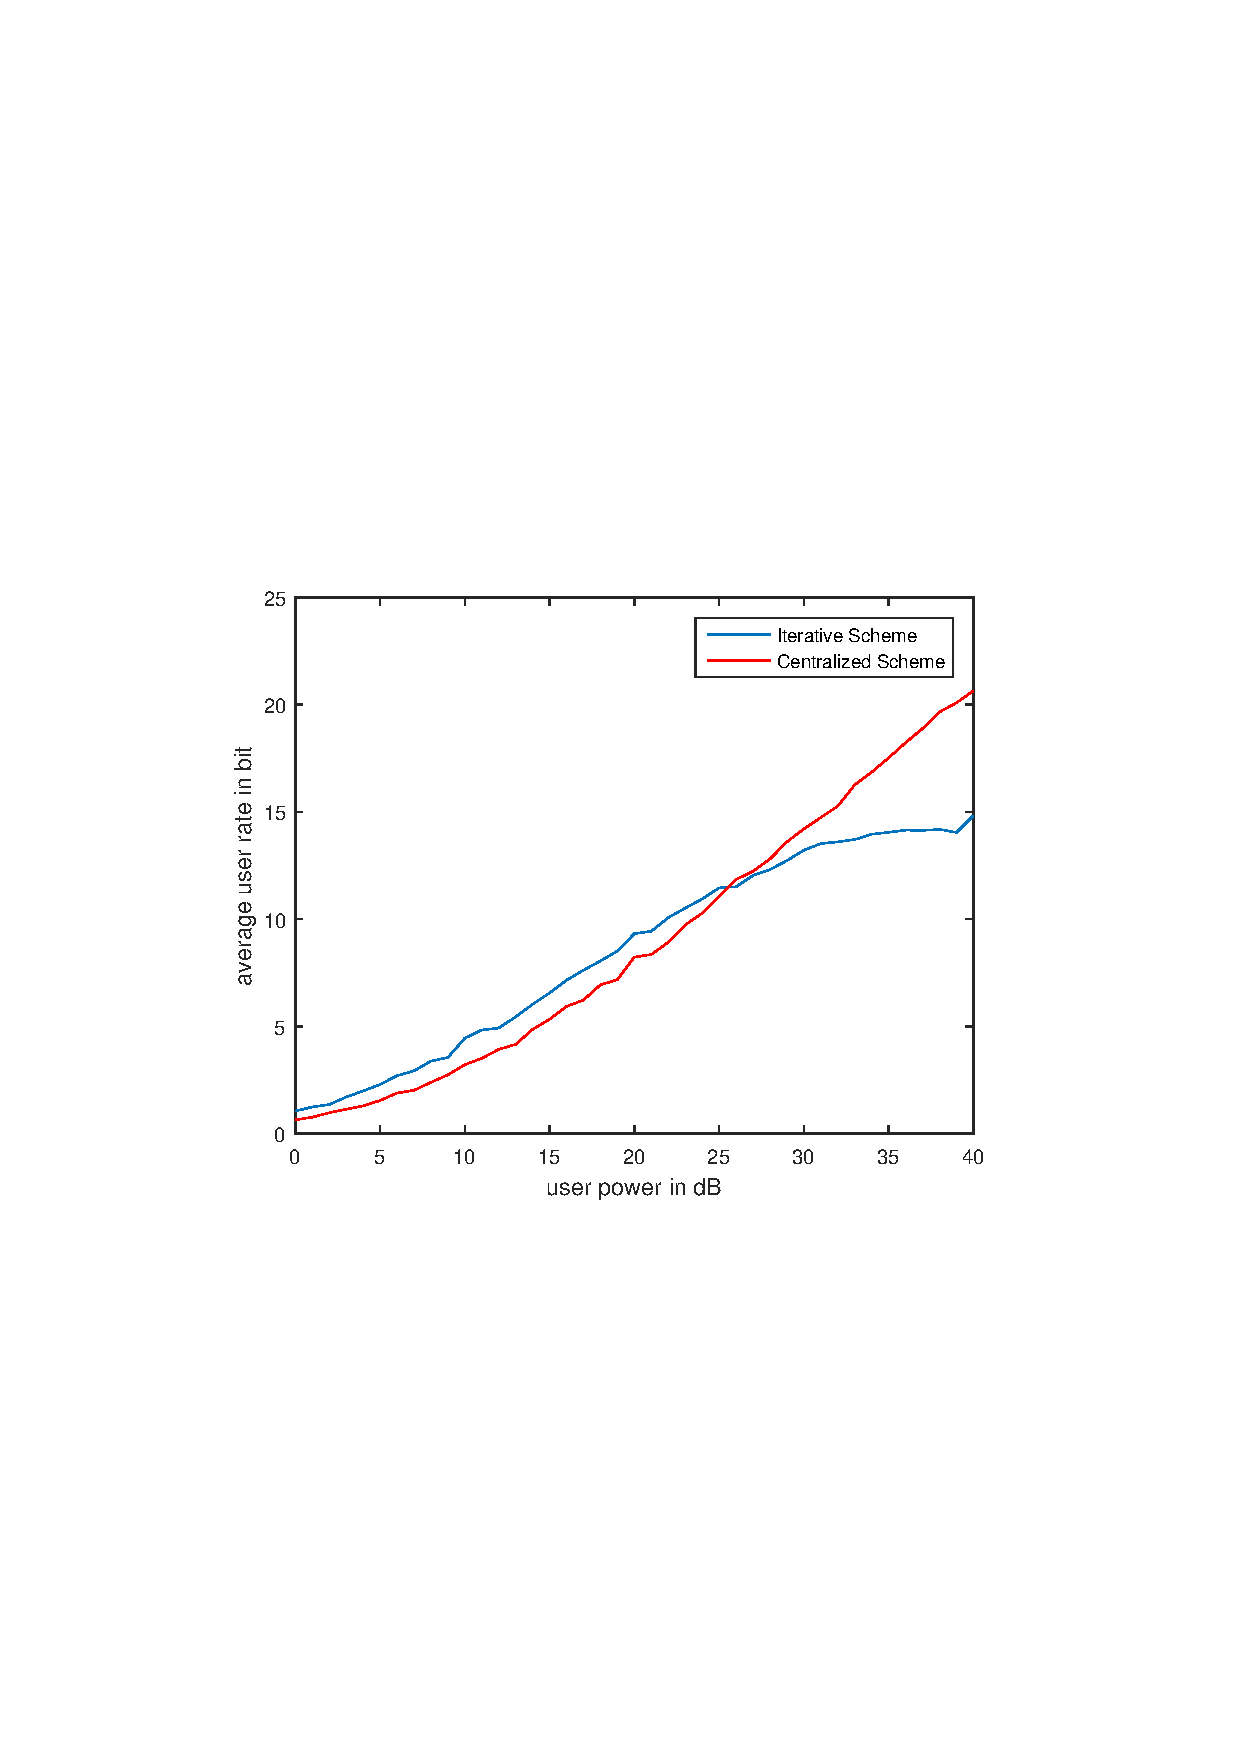
\includegraphics[width=0.65\columnwidth]{result_44.pdf}
    \caption{ Centralized and Distributed Scheme(4,4,2)}\label{FIG:result_44}
\end{figure}
\begin{figure}[H]
    \centering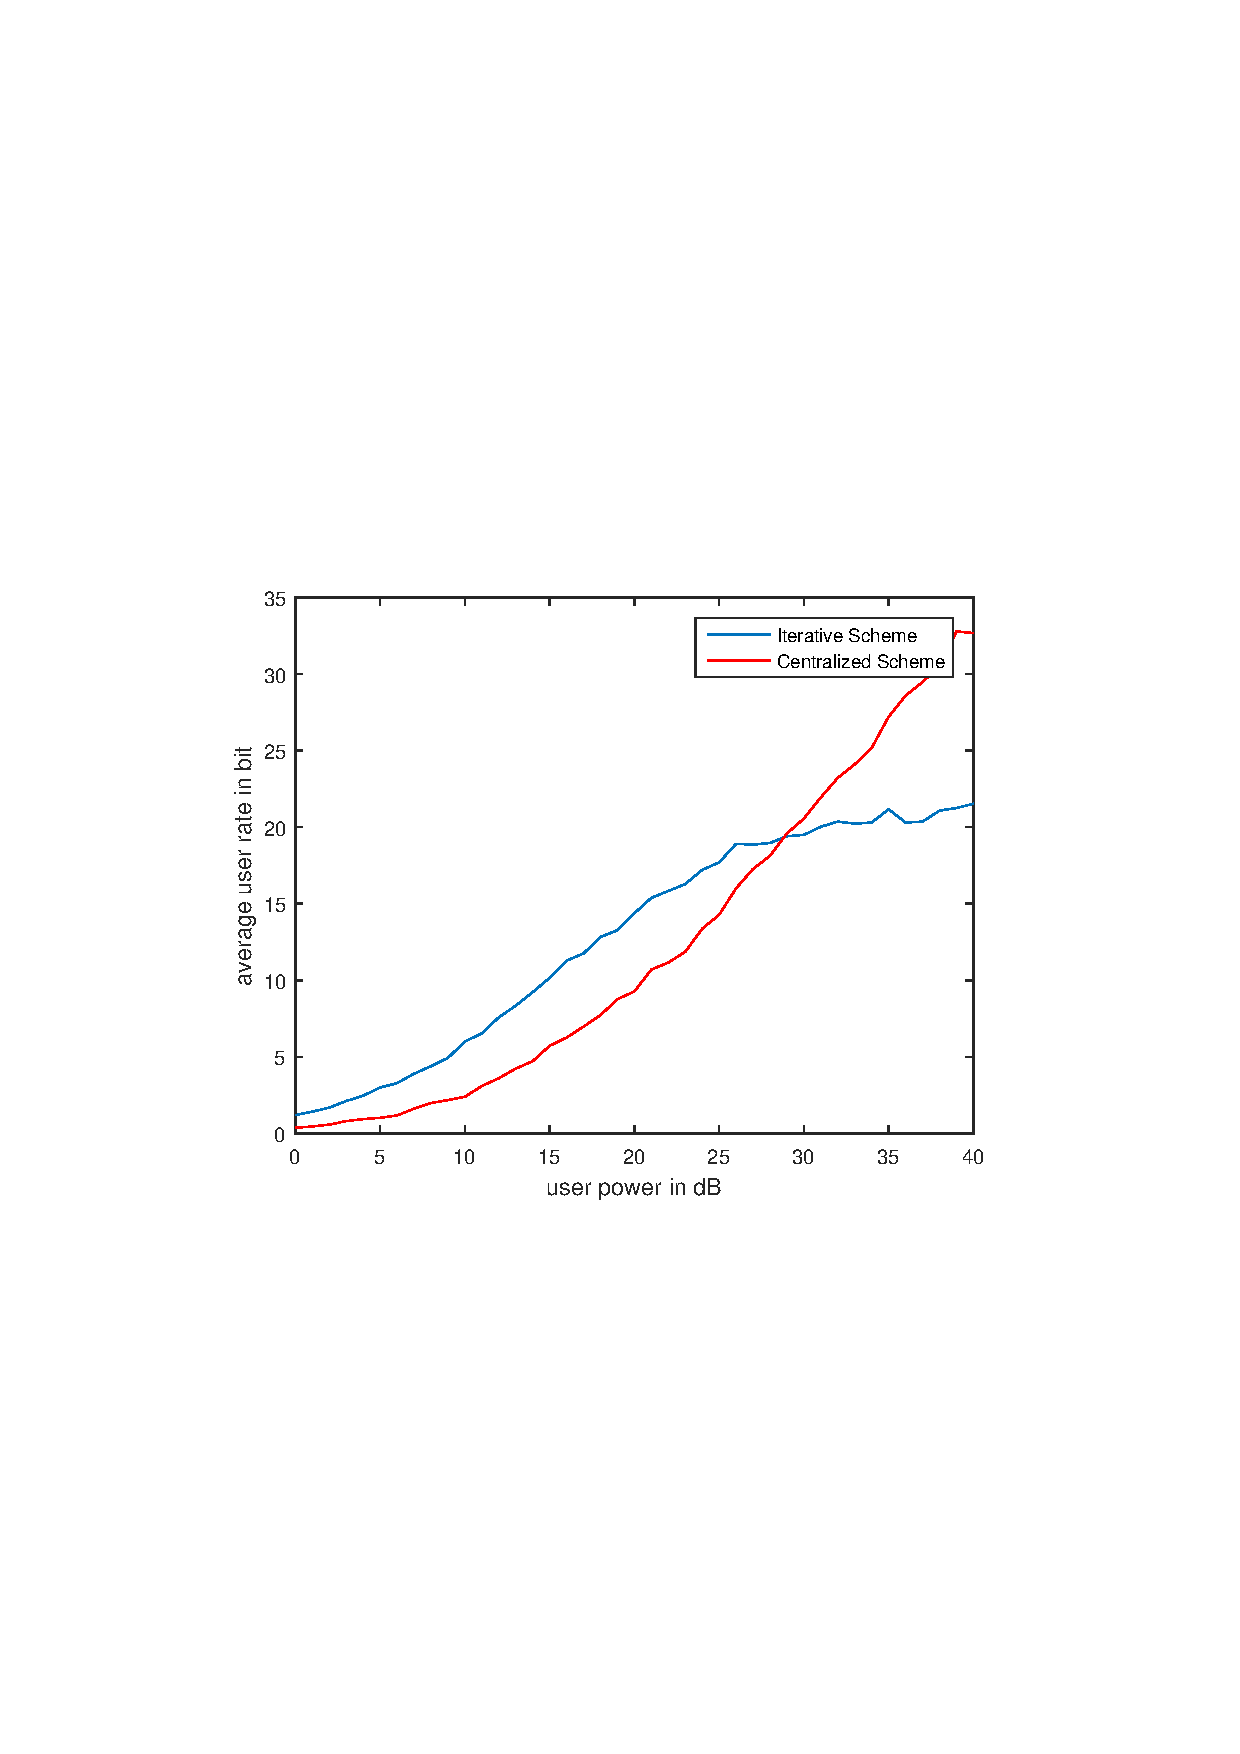
\includegraphics[width=0.65\columnwidth]{result_88.pdf}
    \caption{ Centralized and Distributed Scheme(8,8,4)}\label{FIG:result_88}
\end{figure}


\textbf{As show in Fig.~\ref{FIG:resultWithHeath66.pdf}, we compare the performance of the three IA schemes. }
\begin{figure}[H]
    \centering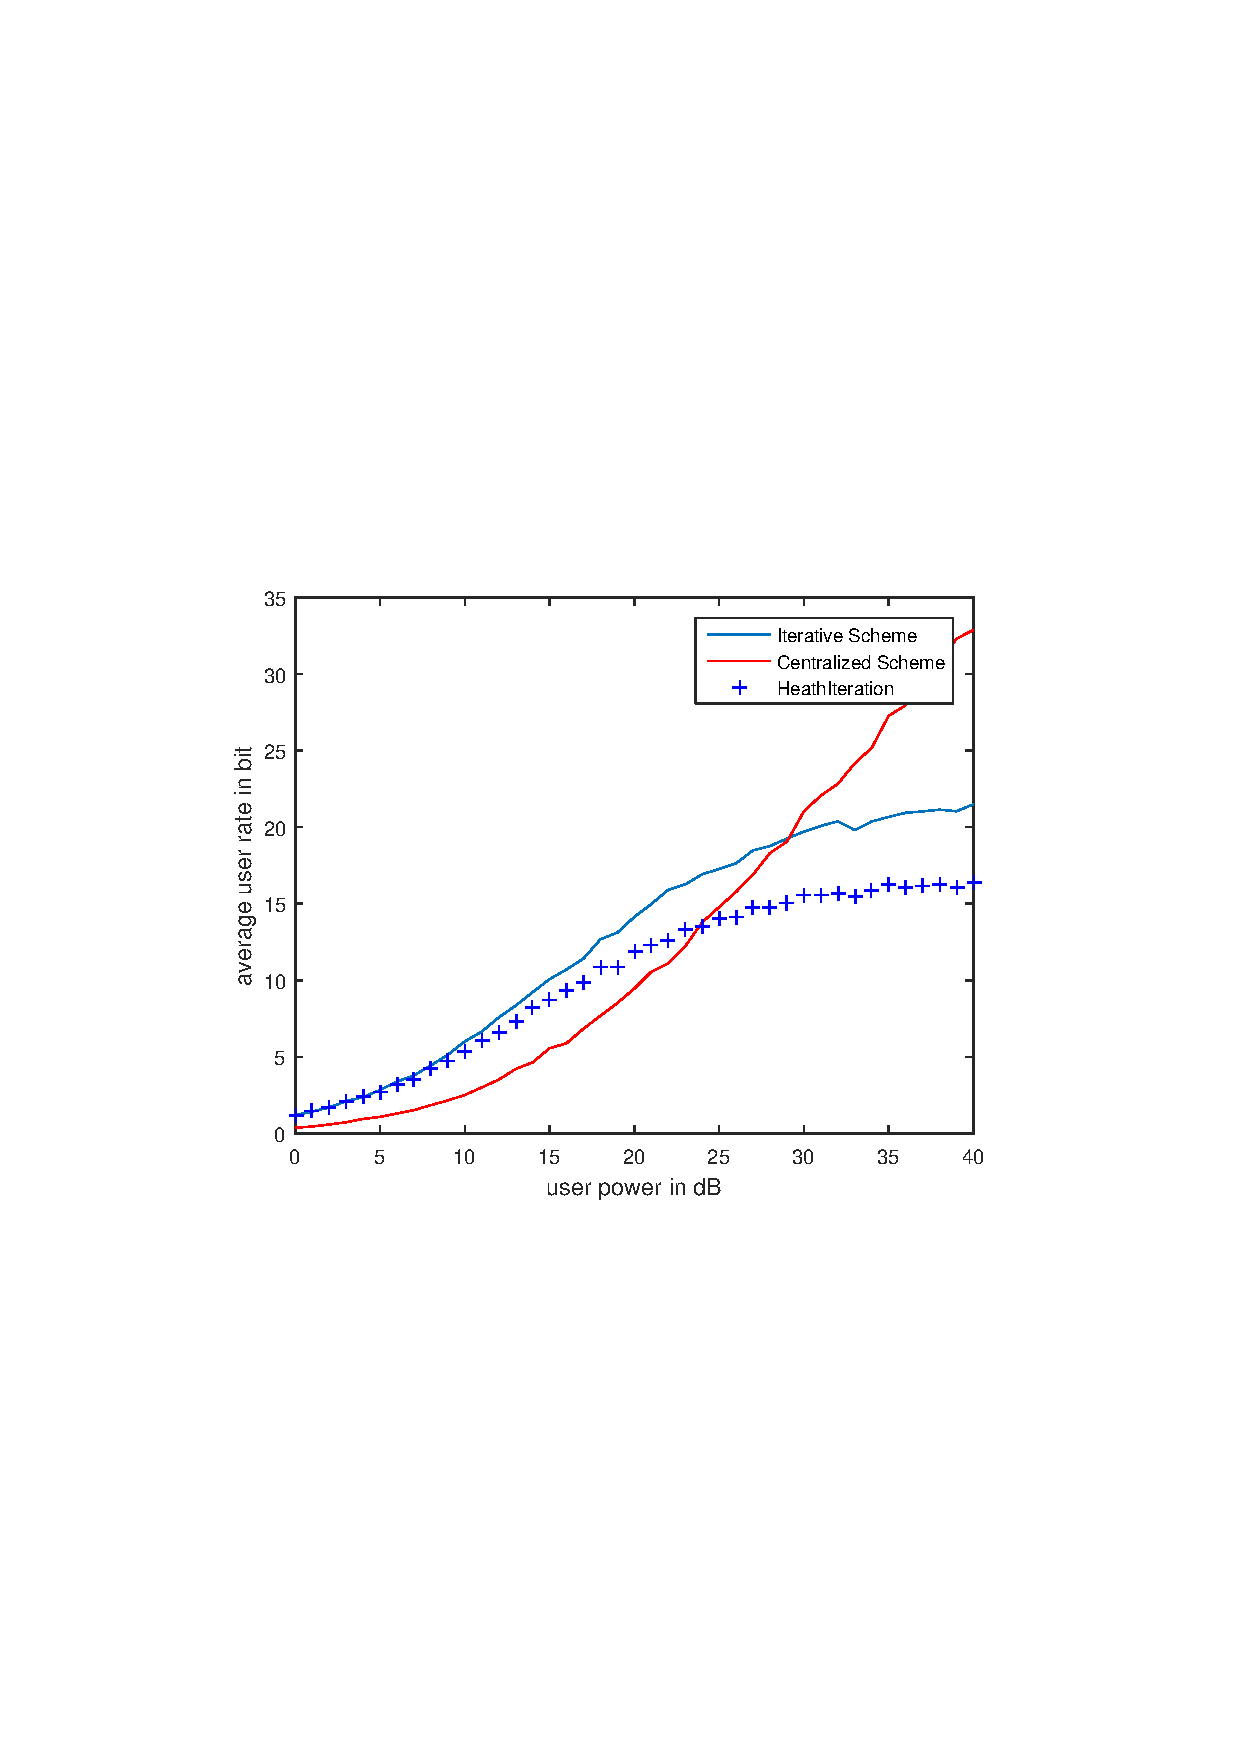
\includegraphics[width=0.65\columnwidth]{resultWithHeath66.pdf}
    \caption{ Centralized , Distributed and Heath Scheme(6,6,3)}\label{FIG:resultWithHeath66.pdf}
\end{figure}



%\bibliographystyle{ieeetr}
\bibliographystyle{hieeetran}
\bibliography{MyCite}
\end{document}
